\documentclass[11pt,a4paper]{article}
\usepackage[utf8]{inputenc}
\usepackage[T1]{fontenc}
\usepackage[margin=18mm,headheight=15pt]{geometry}
\usepackage{lmodern,microtype,xcolor,tikz,tcolorbox,tabularx,array,fancyhdr}
\usetikzlibrary{arrows.meta,positioning}
\definecolor{ink}{HTML}{183149}
\definecolor{blue}{HTML}{2463A6}
\definecolor{teal}{HTML}{087E83}
\definecolor{purple}{HTML}{7449A8}
\definecolor{amber}{HTML}{A65B12}
\definecolor{light}{HTML}{F2F5F8}
\renewcommand{\familydefault}{\sfdefault}
\color{ink}
\setlength{\parindent}{0pt}
\setlength{\parskip}{6pt}
\pagestyle{fancy}\fancyhf{}\fancyhead[L]{\small\textbf{EMPIRIA} / Guía visual del código}\fancyfoot[L]{\small CU-002 + CU-005 · Presentación técnica}\fancyfoot[R]{\thepage}
\renewcommand{\headrulewidth}{0.3pt}
\newcommand{\titulo}[3]{\textcolor{teal}{\small\textbf{#1}}\par{\LARGE\bfseries #2}\par\vspace{2mm}#3\par\vspace{3mm}}
\newcommand{\paso}[4]{\begin{tcolorbox}[colback=#1!5!white,colframe=#1!40!white,boxrule=0.5pt,arc=2mm,left=3mm,right=3mm,top=2mm,bottom=2mm]\textcolor{#1}{\textbf{#2}}\par\textbf{#3}\par #4\end{tcolorbox}}
\newcommand{\nota}[2]{\begin{tcolorbox}[colback=amber!8!white,colframe=amber!40!white,boxrule=0.5pt,arc=2mm]\textcolor{amber}{\textbf{#1}} #2\end{tcolorbox}}
\newcommand{\archivo}[1]{\textbf{#1}}
\newcommand{\met}[1]{\texttt{#1}}
\newcommand{\flecha}{\par\centerline{\textcolor{teal}{\Large$\downarrow$}}\par}
\begin{document}
\raggedright
\titulo{01 / MAPA GENERAL}{Una acción, dos lugares de ejecución}{El navegador muestra la interfaz. Google Apps Script valida y responde. Alpine conecta los datos con lo que ve el usuario.}
\begin{center}
\begin{tikzpicture}[node distance=8mm,>=Latex,every node/.style={font=\small,align=center},box/.style={draw,rounded corners=3mm,text width=135mm,minimum height=17mm,inner sep=3mm}]
\node[box,fill=blue!7,draw=blue] (u) {\textbf{1. USUARIO + VISTA HTML}\\Hace clic, escribe o selecciona una opción.};
\node[box,fill=teal!7,draw=teal,below=of u] (a) {\textbf{2. JAVASCRIPT + ALPINE · NAVEGADOR}\\Cambia el estado y activa la carga.};
\node[box,fill=light,draw=ink!40,below=of a] (p) {\textbf{3. PUENTE · Reactivos.html}\\\texttt{llamarServidor()} utiliza \texttt{google.script.run}.};
\node[box,fill=purple!7,draw=purple,below=of p] (s) {\textbf{4. SERVIDOR GOOGLE · ARCHIVOS .gs}\\Valida parámetros y devuelve datos o un error.};
\node[box,fill=teal!7,draw=teal,below=of s] (r) {\textbf{5. RESPUESTA + STORE + DIRECTIVAS}\\Se actualizan opciones, filas, mensajes y botones.};
\draw[->,thick,blue] (u)--(a);\draw[->,thick,teal] (a)--(p);\draw[->,thick,purple] (p)--(s);\draw[->,thick,teal] (s)--(r);
\end{tikzpicture}
\end{center}
\paso{blue}{AZUL · VISTAS}{Dónde mirar}{\archivo{Index.html, Tareas.html, Reportes.html} y subreportes. Aquí están \met{x-model}, \met{x-for}, \met{x-show} y los eventos.}
\paso{teal}{VERDE · ESTADO Y COORDINACIÓN}{Qué cambia}{\archivo{AlpineTareas.html, AlpineReportes.html, Navegacion.html}, junto con \archivo{Scripts.html} y \archivo{FlujosTareas.html}.}
\paso{purple}{MORADO · SERVIDOR}{Qué se ejecuta en Google}{\archivo{Código.gs, TareasServidor.gs, ReportesServidor.gs} y \archivo{BaseDatos.gs}.}
\nota{Alcance de la entrega.}{La sesión, la publicación de actividades y los datos de reportes son de demostración. Las llamadas al servidor sí atraviesan Apps Script cuando se abre su aplicación web.}
\newpage
\titulo{02 / ARRANQUE Y NAVEGACIÓN}{Cómo aparece la pantalla correcta}{Primero se compone la página en Google. Después, Alpine controla su visibilidad en el navegador.}
\paso{purple}{1 · ABRIR LA URL}{Código.gs → doGet()}{Carga y evalúa \archivo{Index.html}. La función \met{include()} incorpora las vistas y los módulos, incluidas las plantillas anidadas.}
\paso{blue}{2 · RECIBIR EL DOCUMENTO}{Index.html → x-data + carga de Alpine}{El navegador recibe el HTML compuesto. \met{x-data} habilita el ámbito de las directivas. \met{x-cloak}, con su CSS, evita mostrar contenido antes de inicializar Alpine.}
\paso{teal}{3 · INICIALIZAR EL ESTADO}{Evento alpine:init → Alpine.store()}{\archivo{Navegacion.html} registra \met{navegacion}; \archivo{AlpineTareas.html}, \met{tareas}; y \archivo{AlpineReportes.html}, \met{reportes}.}
\paso{teal}{4 · ENTRAR EN LA DEMOSTRACIÓN}{Scripts.html → iniciarSesion(destino)}{Cambia \met{sesionIniciada} a verdadero, prepara plantillas y llama a \met{cargarPlantillas()}. La navegación inicial utiliza \met{switchTab()}.}
\paso{blue}{5 · PULSAR UN MÓDULO}{Index.html → @click}{El botón llama a \met{\$store.navegacion.navegar('tareas')} o a la ruta de reportes.}
\paso{teal}{6 · CAMBIAR Y PREPARAR LA VISTA}{Navegacion.html → navegar(destino)}{Valida el destino y asigna \met{vistaActual}. Los \met{x-show} muestran la vista. \met{Alpine.nextTick()} espera al DOM y ejecuta \met{MODULOS[destino].alEntrar()}, definido en \archivo{Scripts.html}.}
\begin{center}\textcolor{blue}{\textbf{Clic}} $\rightarrow$ \textcolor{teal}{\textbf{vistaActual}} $\rightarrow$ \textcolor{blue}{\textbf{x-show}} $\rightarrow$ \textcolor{teal}{\textbf{alEntrar()}}\end{center}
\nota{Para explicar en voz alta:}{``La vista no se vuelve a descargar al navegar: cambiamos un estado y Alpine muestra el módulo correspondiente''.}
\newpage
\titulo{03 / CU-002 · CATÁLOGO}{Del servidor al selector de plantillas}{Aquí se demuestra el poblamiento con datos remotos mediante \met{x-for}.}
\paso{teal}{1 · ENTRAR EN TAREAS}{Scripts.html → MODULOS.tareas.alEntrar()}{Ejecuta \met{actualizarUICiclo()} y \met{Alpine.store('tareas').cargarPlantillas()}.}
\paso{teal}{2 · ACTIVAR LA CARGA}{AlpineTareas.html → cargarPlantillas(forzar)}{Obtiene el ciclo con \met{cicloReporte()}, evita consultas repetidas y activa \met{cargandoPlantillas}. Incrementa \met{solicitud} para descartar respuestas antiguas.}
\paso{purple}{3 · CONSULTAR GOOGLE}{Reactivos.html → llamarServidor()}{Transmite \met{obtenerPlantillasTarea(ciclo)} mediante \met{google.script.run}. El endpoint está en \archivo{TareasServidor.gs}.}
\paso{teal}{4 · RECIBIR Y PREPARAR}{AlpineTareas.html → cargarPlantillas()}{Valida el ciclo y el catálogo; conserva asociaciones locales. Llama a \met{actualizarSelectPlantillas()} y \met{renderizarPlantillas()}, de \archivo{Scripts.html}. El getter \met{disponibles} filtra las plantillas seleccionables.}
\paso{blue}{5 · GENERAR LAS OPCIONES}{Tareas.html → x-for}{Alpine recorre \met{\$store.tareas.disponibles} y crea una opción por plantilla. El selector usa \met{x-model} para conservar el ID elegido.}
\begin{tcolorbox}[colback=ink,coltext=white,colframe=ink,arc=2mm]
\small\ttfamily
<template x-for="plantilla in \$store.tareas.disponibles"\\
\hspace*{3mm}:key="plantilla.id">\\
\hspace*{3mm}<option :value="plantilla.id"\\
\hspace*{6mm}x-text="plantilla.nombre + plantilla.extension">\\
\hspace*{3mm}</option>\\
</template>
\end{tcolorbox}
\textbf{Lee el fragmento así:} repetir plantilla → identificarla con \met{:key} → asignar su ID con \met{:value} → mostrar el nombre con \met{x-text}.
\nota{Al terminar:}{\met{catch} conserva el error y \met{finally} restaura la carga de la solicitud vigente. \archivo{Tareas.html} muestra el error y permite reintentar.}
\newpage
\titulo{04 / CU-002 · PUBLICACIÓN}{Del formulario a la confirmación}{Alpine refleja el estado. Las funciones JavaScript validan y coordinan la operación.}
\paso{blue}{1 · ESCRIBIR Y ENVIAR}{Tareas.html → x-model / envío del formulario}{Los campos se sincronizan con \met{\$store.tareas.formulario}. El envío llega a \met{crearTarea(e)}, de \archivo{Scripts.html}.}
\paso{teal}{2 · VALIDAR}{Scripts.html → crearTarea(e)}{Evita la recarga y valida título, descripción, fecha, ciclo, plantilla, rango y duplicados. Usa \met{esFechaFutura()}, \met{validarRangoHojas()}, \met{excedeFinCicloEntrega()} y \met{existeTareaMismoNombre()}. Todavía lee varios campos desde el DOM.}
\paso{teal}{3 · INICIAR Y BLOQUEAR}{Scripts.html → iniciarPublicacion(datos)}{Comprueba operaciones en curso, asigna \met{idOperacion} y ejecuta \met{setBotonCreando(true)}. En \archivo{Tareas.html}, \met{:disabled} bloquea controles y \met{x-text} muestra ``Creando tarea…''.}
\paso{teal}{4 · COORDINAR LA TRANSACCIÓN}{FlujosTareas.html → iniciarTransaccion()}{Registra la operación local. \met{procesarPublicacion()} llama a \met{llamarServidor('publicarActividadDemo', ...)} mediante \archivo{Reactivos.html}.}
\paso{purple}{5 · VALIDAR EN GOOGLE}{TareasServidor.gs → publicarActividadDemo()}{Revalida parámetros. \met{conRegistroDemo\_()} coordina bloqueo y caché. El \met{idOperacion} permite recuperar un resultado previo al reintentar. Devuelve estado, ID y \met{simulacion: true}.}
\paso{teal}{6 · RESOLVER Y CONFIRMAR}{FlujosTareas.html → resolverRespuestaPublicacion()}{Valida la respuesta y decide éxito, error, reintento o cancelación. En éxito, \met{completarPublicacionTransaccion()} actualiza la tarea local, la plantilla y el mensaje; \met{setBotonCreando(false)} restaura el botón.}
\nota{Qué ve el usuario:}{Formulario → ``Creando tarea…'' → confirmación. La publicación es simulada; no crea una tarea real en Classroom. El formulario se limpia al aceptar la confirmación.}
\vspace{5mm}
\begin{center}
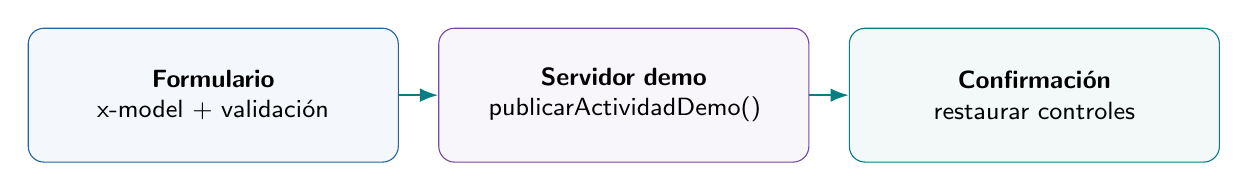
\begin{tikzpicture}[>=Latex,node distance=5mm,every node/.style={font=\small,align=center},b/.style={rounded corners=2mm,draw,text width=43mm,minimum height=17mm,inner sep=2mm}]
\node[b,draw=blue,fill=blue!5] (a) {\textbf{Formulario}\\x-model + validación};
\node[b,draw=purple,fill=purple!5,right=of a] (b) {\textbf{Servidor demo}\\publicarActividadDemo()};
\node[b,draw=teal,fill=teal!5,right=of b] (c) {\textbf{Confirmación}\\restaurar controles};
\draw[->,thick,teal] (a)--(b);\draw[->,thick,teal] (b)--(c);
\end{tikzpicture}
\end{center}
\newpage
\titulo{05 / CU-005 · CONSULTA}{De BaseDatos.gs a las filas del reporte}{La consulta inicial obtiene el conjunto. Los selectores y publicaciones se construyen a partir del estado recibido.}
\paso{teal}{1 · ENTRAR Y CARGAR}{Scripts.html → inicializarModuloReportes()}{Delega en \met{Alpine.store('reportes').cargar()}. En \archivo{AlpineReportes.html}, \met{cargar(forzar)} activa \met{cargando}, limpia el error y llama a \met{establecerPanelesReportes(false)}.}
\paso{purple}{2 · CONSULTAR Y VALIDAR}{Reactivos.html → ReportesServidor.gs}{\met{llamarServidor('obtenerDatosReportes', ...)} llega a \met{obtenerDatosReportes(opciones)}. Lee \met{BASE\_DATOS\_EMPIRIA}, de \archivo{BaseDatos.gs}, y valida sus colecciones.}
\paso{teal}{3 · GUARDAR Y PREPARAR}{AlpineReportes.html → renderizarVistaReportes()}{Guarda la respuesta en \met{datos}. \met{renderizarVistaReportes()}, de \archivo{Scripts.html}, prepara filtros e investigadores, llama a \met{llenarSelectReporte()}, \met{filtrarInvestigadoresReporte()} y \met{cambiarCarreraReporte()}, entre otros.}
\paso{teal}{4 · ACTUALIZAR LAS OPCIONES}{Scripts.html → llenarSelectReporte()}{Delega en \met{llenarSelector()}, del store de \archivo{AlpineReportes.html}. Actualiza \met{opciones}, \met{filtros} y \met{sinOpciones}. Las vistas \archivo{ReporteInvestigador.html} y \archivo{ReporteCarrera.html} usan \met{x-for} y \met{x-model}.}
\paso{teal}{5 · PREPARAR LAS FILAS}{Scripts.html → renderizarColeccionInv(tipo)}{Obtiene la página con \met{paginaColeccionInv(tipo)}. Para publicaciones actualiza columnas y filas de \met{\$store.reportes.tablas[tipo]}.}
\paso{blue}{6 · DIBUJAR Y MOSTRAR}{TablaPublicaciones.html → x-for}{Genera cabeceras, filas y columnas. \met{x-html} muestra las celdas de \met{celdaColeccionInv()}, que escapa texto y valida enlaces. Después de \met{Alpine.nextTick()}, se muestran los paneles y \met{finally} desactiva la carga.}
\begin{center}\textcolor{purple}{\textbf{Datos}} $\rightarrow$ \textcolor{teal}{\textbf{store}} $\rightarrow$ \textcolor{teal}{\textbf{columnas + filas}} $\rightarrow$ \textcolor{blue}{\textbf{x-for}}\end{center}
\newpage
\titulo{06 / INTERACCIÓN Y RECUPERACIÓN}{Qué ocurre después de la carga}{Buscar, cambiar de reporte y recuperarse de un error son recorridos distintos.}
\paso{blue}{BUSCAR PUBLICACIONES}{Scripts.html → buscarColeccionInv(tipo, valor)}{Actualiza la búsqueda y llama a \met{renderizarColeccionInv(tipo)}. Se recalculan las filas y Alpine actualiza la tabla. \textbf{No se consulta de nuevo al servidor}: se trabaja con los datos recibidos.}
\paso{teal}{CAMBIAR INVESTIGADOR / CARRERA}{Reportes.html → Navegacion.html}{El botón usa \met{@click} para llamar a \met{cambiarReporte(nombre)}. El método valida el nombre, cambia \met{reporteActual} y los \met{x-show} presentan el subreporte seleccionado.}
\paso{amber}{ERROR EN REPORTES}{AlpineReportes.html → catch / finally}{\met{catch} limpia los datos y guarda el mensaje. \met{finally} desactiva \met{cargando}. En \archivo{Reportes.html}, el botón ejecuta \met{\$store.reportes.cargar(true)} para reintentar.}
\paso{amber}{ERROR O CANCELACIÓN DE PUBLICACIÓN}{FlujosTareas.html → resolverRespuestaPublicacion()}{Clasifica el error. Las cuotas admiten hasta tres reintentos con espera progresiva; el fallo definitivo se gestiona con \met{fallarTransaccion()}. La interfaz permanece en proceso mientras se resuelve la operación.}
\paso{teal}{CANCELAR LA OPERACIÓN}{FlujosTareas.html → marcarCancelacionPublicacion()}{El recorrido de \met{cancelarPublicacionEnCurso()} utiliza \met{cancelarActividadDemo()}, de \archivo{TareasServidor.gs}. El estado \met{cancelando} coordina la acción y evita que una respuesta tardía confirme una operación cancelada.}
\nota{Diferencia clave:}{Reportes restaura su carga en \met{finally}. Publicación también coordina transacciones, reintentos y cancelación; su finalización no se reduce a un único \met{finally}.}
\textbf{Prueba para la exposición:} en Condiciones de prueba selecciona ``Repositorio no disponible'', muestra el error, restaura ``Disponible'' y pulsa Reintentar. Comprueba la URL de Apps Script antes de presentar.
\newpage
\titulo{07 / CHULETA PARA EXPONER}{Directiva → efecto visible → archivo}{Usa esta página para conectar cada concepto con una parte concreta del recorrido.}
\renewcommand{\arraystretch}{1.55}
\begin{tabularx}{\textwidth}{>{\bfseries\color{teal}}p{25mm} X p{48mm}}
Directiva & Efecto que debes señalar & Archivo de referencia\\\hline
\met{x-data} & Habilita el ámbito de Alpine. & Index.html\\
\met{x-model} & Sincroniza campo y estado en ambos sentidos. & Tareas.html\\
\met{x-for} & Genera opciones y filas desde colecciones. & Tareas.html / TablaPublicaciones.html\\
\met{:key} & Identifica los elementos de una iteración. & TablaPublicaciones.html\\
\met{x-text} & Cambia nombres, mensajes y texto del botón. & Tareas.html / Reportes.html\\
\met{x-show} & Muestra u oculta vistas o mensajes. & Tareas.html / Reportes.html\\
\met{:disabled} & Bloquea controles durante una operación. & Tareas.html\\
\met{@click} & Atiende el clic e inicia una acción. & Index.html / Reportes.html\\
\met{:value} & Asigna el valor de cada opción. & Tareas.html\\
\met{x-html} & Presenta las celdas HTML preparadas. & TablaPublicaciones.html\\
\met{x-cloak} & Oculta contenido antes de inicializar Alpine. & Tareas.html\\
\end{tabularx}
\vspace{5mm}
\paso{teal}{FRASE PARA EXPLICAR EL MECANISMO}{``Cambiamos el estado; Alpine actualiza la vista''}{\met{\$store} permite acceder al estado compartido: no es una directiva. \met{:disabled} y \met{:value} son usos de \met{x-bind}; \met{@click} es la abreviatura de \met{x-on:click}.}
\nota{Límites que debes declarar:}{El login es simulado; los reportes usan datos demo y la publicación no llega a Classroom. Otros gráficos y listados conservan renderizadores tradicionales. La integración real y la validación remota completa siguen pendientes.}
\end{document}
